\section{Results}\label{sec:results}

\subsection{Carbon-intensity data and forecasts}\label{sec:res_forecast}

Fig.~\ref{fig:data} shows the regional intensities. Over 2022--2024, mean intensity was 37~gCO$_2$/kWh in South Scotland, 58 in North West England, 156 in the West Midlands and 163 in London. At any hour the gap between the cleanest and dirtiest site is therefore large, which is what makes spatial shifting attractive. Intensities fell steadily: London's annual mean dropped from 202~gCO$_2$/kWh in 2022 to 124 in 2024. Diurnal profiles peak in the early evening (around 18:00 UTC), and the profile of South Scotland is much flatter than those of the southern sites. The four series are positively correlated (pairwise correlations between 0.50 and 0.87), because national wind output drives all of them.

\begin{figure}[t]
\centering
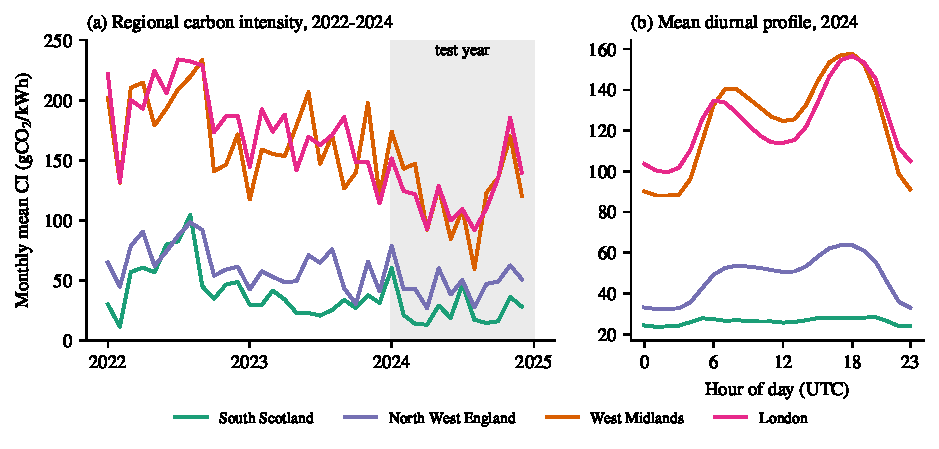
\includegraphics[width=\textwidth]{../figures/fig2_data.pdf}
\caption{Hourly carbon intensity of the four candidate sites (NESO regional data). (a) Monthly means, 2022--2024; the shaded area is the out-of-sample test year. (b) Mean diurnal profile in 2024 (UTC).}
\label{fig:data}
\end{figure}

Table~\ref{tab:forecast} and Fig.~\ref{fig:forecast}a summarise forecast accuracy in 2024. The forecaster was trained on 1.24 million (issue time, site, horizon) samples in about one minute. Averaged over horizons and sites, the direct GBM forecaster has a mean absolute error (MAE) of 31.2~gCO$_2$/kWh, against 34.4 for persistence and 40.4 for the seasonal-naive forecast. The advantage is largest at short and medium horizons: MAE falls by 23\% at 1 hour (6.2 against 8.0) and by 23\% at 6 hours (23.3 against 30.2). Beyond about 18 hours, all methods converge to the seasonal-naive level, and at 24 hours the GBM is slightly worse than the seasonal-naive benchmark. Without weather forecasts, day-ahead changes in wind output are hard to predict from the intensity history alone~\cite{maji2022carboncast}. By site, the GBM is most accurate for the volatile southern sites. In South Scotland, where intensity is low and often flat, persistence is marginally better.

\begin{table}[t]
\centering
\caption{Forecast accuracy on the 2024 test year (MAE in gCO$_2$/kWh; mean over sites unless stated).}
\label{tab:forecast}
\small
\begin{tabular}{lrrrrrrr}
\toprule
 & \multicolumn{5}{c}{Horizon $h$ (hours)} & \multicolumn{2}{c}{All horizons} \\
\cmidrule(lr){2-6}\cmidrule(lr){7-8}
Model & 1 & 3 & 6 & 12 & 24 & MAE & RMSE \\
\midrule
Persistence & 8.0 & 19.3 & 30.2 & 37.4 & 40.4 & 34.4 & 48.4 \\
Seasonal naive (24 h) & 40.4 & 40.4 & 40.4 & 40.4 & 40.4 & 40.4 & 57.0 \\
Direct GBM (this study) & \textbf{6.2} & \textbf{14.9} & \textbf{23.3} & \textbf{33.9} & 42.4 & \textbf{31.2} & \textbf{41.0} \\
\bottomrule
\end{tabular}

\smallskip
\parbox{0.92\textwidth}{\footnotesize MAE by site over all horizons (persistence / GBM): South Scotland 14.1 / 16.2; North West England 24.7 / 21.8; West Midlands 56.1 / 49.3; London 42.7 / 37.6.}
\end{table}

\begin{figure}[t]
\centering
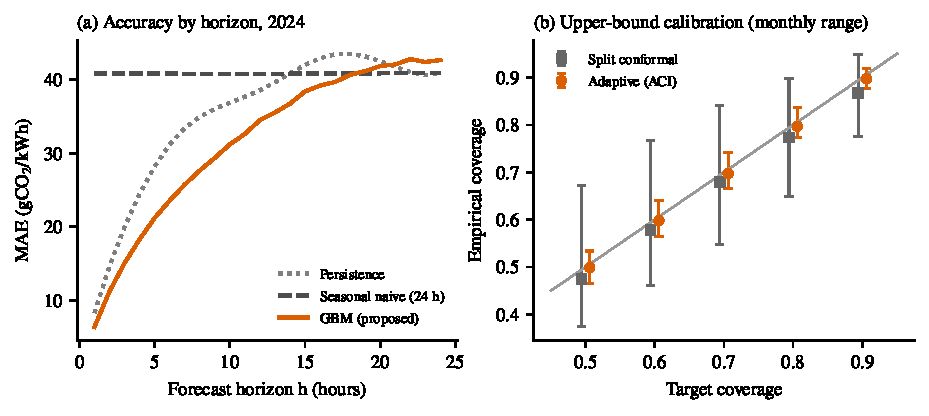
\includegraphics[width=\textwidth]{../figures/fig3_forecast.pdf}
\caption{Forecast evaluation in 2024. (a) MAE by horizon, averaged over sites. (b) Empirical coverage of one-sided upper bounds $U^\beta$ against the target level $\beta$ for static split conformal calibration and adaptive conformal inference (ACI). Markers show the annual coverage and bars the range across the 12 months.}
\label{fig:forecast}
\end{figure}

Calibration matters more than point accuracy for the risk-adjusted cost view, and Fig.~\ref{fig:forecast}b shows the effect of distribution shift. Static split-conformal bounds, calibrated on July--September 2023, under-cover in 2024 at every level: at $\beta=0.9$, annual coverage was 0.858 and monthly coverage ranged from 0.68 to 0.95. With ACI, annual coverage matches the target to within 0.002 at all levels (0.500, 0.599, 0.698, 0.798 and 0.898). Monthly coverage stays within $\pm 4$ percentage points of the target, and coverage is uniform across horizons. At $\beta=0.5$, the ACI-adjusted median lies on average 9.9~gCO$_2$/kWh below the point forecast, which reflects the downward drift in intensity that the static model does not capture.

\subsection{Hyperparameter tuning}\label{sec:tuning}

Fig.~\ref{fig:tuning} reports the validation results (13 weeks, October--December 2023, $\rho\in\{0.3,0.5,0.7\}$, migration allowed). Anticipating demand helps across the whole grid: every tested configuration beats myopic MPC, whose mean gap to the oracle is 20.3\%. The gap is smallest around $\kappa=1$, where expected demand is anticipated without inflation. For $\ell=12$ it falls to 7.3\%, and for $\ell=18$ to 7.2\%. Over-anticipation ($\kappa=1.25$ with $\ell=18$) reserves too much clean capacity and is penalised. We selected $\kappa=1$ and $\ell=12$ hours. Configurations within 0.25 percentage points of the best were resolved towards the shorter look-ahead, which keeps the network smaller.

\begin{figure}[t]
\centering
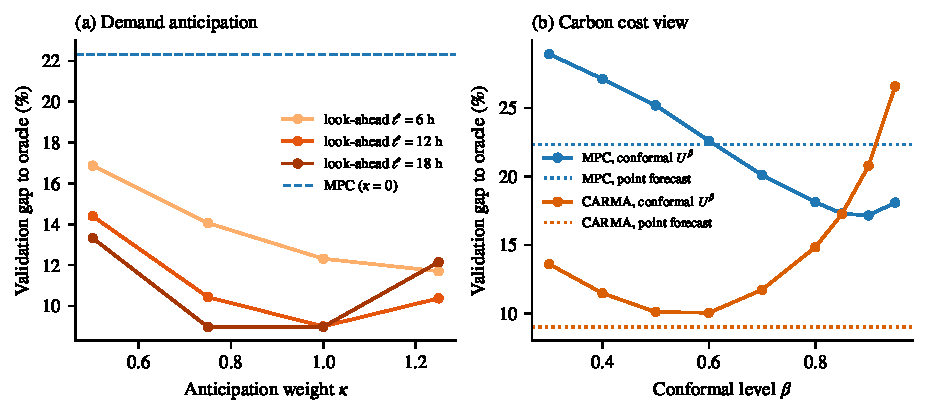
\includegraphics[width=\textwidth]{../figures/fig6_tuning.pdf}
\caption{Validation results (2023-Q4, mean over 13 weeks and three load levels). (a) Gap to the oracle as a function of the anticipation weight $\kappa$ and look-ahead $\ell$, using point forecasts. (b) Effect of the carbon cost view: conformal upper quantiles $U^\beta$ against point forecasts, for myopic MPC and for CARMA ($\kappa=1$, $\ell=12$).}
\label{fig:tuning}
\end{figure}

The cost view shows a clear interaction with anticipation (Fig.~\ref{fig:tuning}b). For myopic MPC, pessimistic conformal costs help substantially. The gap falls monotonically from 23.1\% at $\beta=0.5$ to 16.2\% at $\beta=0.8$, well below the 20.3\% obtained with point forecasts. For CARMA, every conformal level is worse than the point forecast: the best level, $\beta=0.6$, gives 8.2\% against 7.3\%. The explanation is that a risk premium on future hours makes the planner run work now rather than later, which keeps future clean capacity free. For a myopic planner this is a crude form of anticipation. Once CARMA represents future demand explicitly, the same premium double-counts it and gives up useful deferrals. The selected CARMA therefore uses point forecasts. For the test we keep MPC+conformal at $\beta=0.8$ and CARMA+conformal at $\beta=0.6$ as ablations.

\subsection{Out-of-sample scheduling performance}\label{sec:res_main}

Tables~\ref{tab:main} and~\ref{tab:main_t} report results for the 52 test weeks of 2024. Weekly traces contain on average 920, 1{,}529 and 2{,}144 jobs (69{,}900, 115{,}600 and 162{,}600 server-hours) at $\rho=0.3$, 0.5 and 0.7. Fig.~\ref{fig:gap} shows the gaps to the oracle with 95\% confidence intervals.

\begin{table}[p]
\centering
\caption{Out-of-sample results in the spatio-temporal regime (migration allowed), 52 weeks of 2024. Emis.: mean weekly operational emissions (tCO$_2$). Red.: reduction relative to ASAP-Local (\%). Gap: excess over the clairvoyant oracle (\%). Late: share of work finished after its deadline (\%). Mig.: share of work executed away from its origin (\%). $p$: Holm-adjusted two-sided Wilcoxon signed-rank test of weekly emissions against CARMA. The best gap among implementable online policies is in bold.}
\label{tab:main}
\footnotesize
\begin{tabular}{llrrrrrl}
\toprule
Load & Policy & Emis. & Red. & Gap & Late & Mig. & $p$ \\
\midrule
\inputtable{../results/table_main_st.tex}
\bottomrule
\end{tabular}
\end{table}

\begin{table}[p]
\centering
\caption{Out-of-sample results in the temporal-only regime (no migration), 52 weeks of 2024. Columns as in Table~\ref{tab:main}. Greedy-Spatial is omitted because without migration it coincides with ASAP-Local.}
\label{tab:main_t}
\footnotesize
\begin{tabular}{llrrrrl}
\toprule
Load & Policy & Emis. & Red. & Gap & Late & $p$ \\
\midrule
\inputtable{../results/table_main_t.tex}
\bottomrule
\end{tabular}
\end{table}

\begin{figure}[t]
\centering
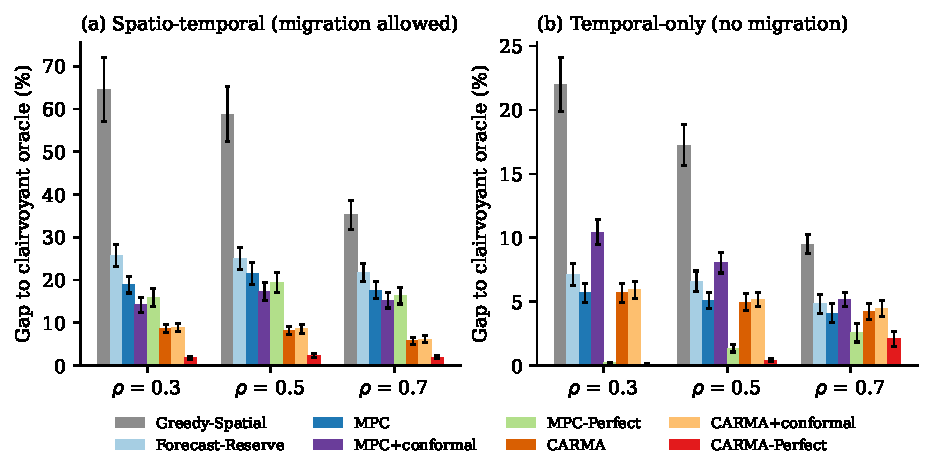
\includegraphics[width=\textwidth]{../figures/fig4_gap.pdf}
\caption{Mean gap to the clairvoyant oracle over the 52 test weeks of 2024 with 95\% confidence intervals. ASAP-Local is omitted (gap 68--275\% with migration, 9--22\% without).}
\label{fig:gap}
\end{figure}

\paragraph{Spatio-temporal regime} Carbon-aware scheduling gives large reductions when migration is allowed. The oracle cuts emissions relative to ASAP-Local by 70.5\%, 56.7\% and 39.5\% at $\rho=0.3$, 0.5 and 0.7. The achievable reduction shrinks with load because less clean capacity is left per unit of work. Greedy-Spatial realises only part of this potential (gaps of 35--65\%), because it has no temporal flexibility and floods the cleanest site with whatever arrives first. Forecast-Reserve and MPC come closer, with gaps of 18--26\%. CARMA reduces emissions by 68.1\%, 53.3\% and 36.1\% and reaches gaps of 8.7\%, 8.2\% and 5.8\%. Relative to MPC this is a further emission reduction of 7.6\%, 9.4\% and 8.8\%, and the gap to the optimum shrinks by a factor of 2.2--3.0. CARMA's emissions are lower than MPC's in 51, 52 and 52 of the 52 weeks, and lower than Forecast-Reserve's in every week (Fig.~\ref{fig:weekly}b). All differences between CARMA and the online baselines are significant after Holm correction ($p<0.001$). The only exception is CARMA+conformal at $\rho=0.3$ ($p=0.12$). CARMA also finishes more work on time under heavy load: at $\rho=0.7$, 0.05\% of its work is late, against 2.0\% for MPC, 1.2\% for Forecast-Reserve and 6.5\% for ASAP-Local. Reserving clean capacity for urgent arrivals also reserves capacity in general. CARMA migrates about the same share of work as MPC (31--70\%), so its advantage comes from better timing of the use of scarce clean capacity, not from moving more data. For a fleet of 1{,}700 batch servers at $\rho=0.5$, the difference between CARMA and MPC is 0.31~tCO$_2$ per week. The difference from carbon-agnostic operation is 3.16~tCO$_2$ per week.

\begin{figure}[t]
\centering
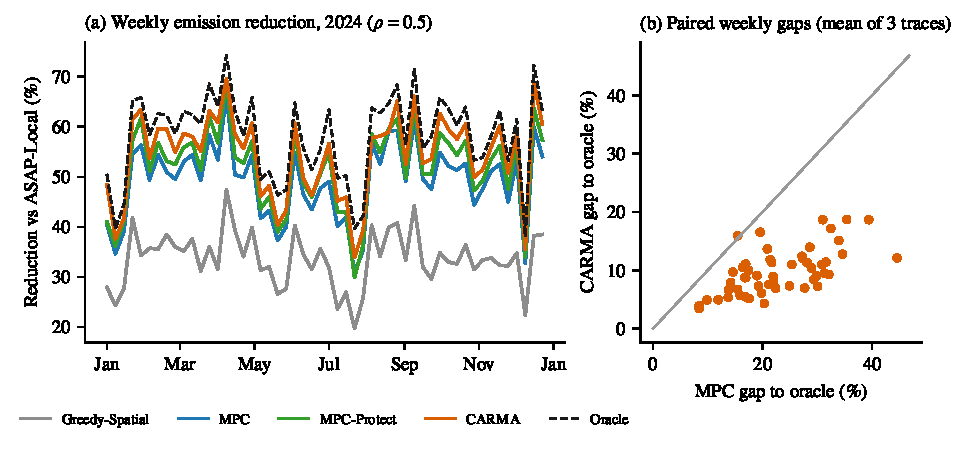
\includegraphics[width=\textwidth]{../figures/fig5_weekly.pdf}
\caption{Weekly results in 2024 (spatio-temporal regime, $\rho=0.5$). (a) Emission reduction relative to ASAP-Local. (b) Paired weekly gaps to the oracle; points below the diagonal are weeks in which CARMA outperforms MPC.}
\label{fig:weekly}
\end{figure}

\paragraph{Value of information} The clairvoyant variants separate two sources of loss. With perfect intensity forecasts, the myopic MPC-Perfect still has gaps of 15.9\%, 19.5\% and 16.3\%. Perfect carbon foresight is thus worth only 1.3--3.0 percentage points to a myopic planner. Anticipating demand is worth 10.3--13.3 points (MPC versus CARMA). With both, CARMA-Perfect comes within 1.8--2.3\% of the oracle. The two kinds of information are therefore complementary. Once demand is anticipated, forecast accuracy is worth 3.9--6.8 points (CARMA versus CARMA-Perfect), two to three times more than for the myopic planner. A myopic planner wastes clean capacity whatever its forecasts, so it cannot benefit from better ones. The weekly results in Fig.~\ref{fig:weekly}a show that the ranking is stable across seasons, although the level of achievable reductions varies from week to week with wind conditions.

\paragraph{Temporal-only regime} Without migration (Table~\ref{tab:main_t}), each job can only move in time at its origin, and the picture changes. Achievable reductions are much smaller: the oracle saves 17.7\%, 14.5\% and 8.6\%. MPC and CARMA are statistically indistinguishable here ($p\ge 0.22$), both about 4--6\% from the oracle, and both are better than Forecast-Reserve. Anticipation brings no benefit because there is no shared pool of clean capacity to protect. Each site's capacity serves only its own jobs, and the temporal windows of flexible jobs rarely collide with urgent arrivals in a way that deferral cannot absorb. In this regime the remaining loss is due almost entirely to forecast error. MPC-Perfect and CARMA-Perfect close the gap to 0.1--2.6\%, and risk-averse conformal costs make MPC worse (gaps of 5.2--10.4\%), because they suppress deferrals that would have paid off. Under heavy load ($\rho=0.7$), temporal shifting also raises lateness: the capacity at the origin sites is itself insufficient, and 6.5\% of work is late even under ASAP-Local. CARMA's late share (6.9\%) is close to that level, whereas MPC's is 13.0\%.

\paragraph{Computation} A CARMA decision takes 20--47~ms on one CPU core, against 2--7~ms for MPC. The difference comes from the ghost jobs, which enlarge the planning network. This is negligible for hourly decisions. A clairvoyant weekly oracle with up to about 2{,}700 jobs (including warm-up and trailing load) is solved exactly in under one second.

\subsection{Sensitivity analysis}\label{sec:sens}

Table~\ref{tab:sens} varies one factor at a time around the base case: spatio-temporal regime, $\rho=0.5$, $\upsilon=0.3$, $\eta=0.02$~kWh/GB. Each setting uses 26 alternating test weeks of 2024 with fresh workload seeds. CARMA keeps its hyperparameters from the base case. CARMA has the smallest gap of all online policies in every setting. Its weekly emissions are below MPC's in 155 of the 156 setting-weeks, and every comparison with a baseline is significant (all $p<10^{-7}$).

\begin{table}[t]
\centering
\caption{Sensitivity analysis (spatio-temporal regime; 26 alternating weeks of 2024 per setting; base case $\rho=0.5$, $\upsilon=0.3$, $\eta=0.02$~kWh/GB). Oracle red.: emission reduction of the oracle relative to ASAP-Local (\%). Gap columns: excess over the oracle (\%). Wins: weeks in which CARMA emits less than MPC. Late: share of late work (\%), MPC / CARMA.}
\label{tab:sens}
\footnotesize
\resizebox{\textwidth}{!}{%
\begin{tabular}{lrrrrrrr}
\toprule
 & Oracle & \multicolumn{4}{c}{Gap to oracle (\%)} & Wins vs & Late (\%) \\
\cmidrule(lr){3-6}
Setting & red. & Greedy-Sp. & F.-Reserve & MPC & CARMA & MPC & MPC / CARMA \\
\midrule
\inputtable{../results/table_sens.tex}
\bottomrule
\end{tabular}}
\end{table}

\paragraph{Share of urgent jobs} The benefit of anticipation grows with the share of urgent work, because urgent arrivals are precisely the demand that myopic planners crowd out. With $\upsilon=0.5$, CARMA's gap is 5.8\% against 20.3\% for MPC, and it has no late work (MPC 0.15\%). With $\upsilon=0.1$, the gap is 10.4\% against 20.9\%. When almost all work is flexible, there is less urgent demand to protect capacity for.

\paragraph{Network energy intensity} The ranking is unchanged over a twelve-fold range of transmission energy intensity. Cheaper transfers ($\eta=0.005$~kWh/GB) raise the oracle's reduction to 60.7\%, and CARMA's gap is 9.4\% against 25.0\% for MPC. Expensive transfers ($\eta=0.06$~kWh/GB) lower the oracle's reduction to 52.3\%, with gaps of 7.4\% and 18.1\%. The share of migrated work changes only modestly (49--51\% for CARMA), because the intensity difference between South Scotland and London is far larger than any plausible transfer overhead.

\paragraph{Misspecified demand profile} CARMA's ghost jobs come from a profile learned at $\rho=0.5$. When the actual load is 20\% higher ($\rho=0.6$), so that CARMA under-anticipates, its gap is 6.9\% against 22.1\% for MPC, and its late share is 0.01\% against 0.34\%. When the actual load is 20\% lower ($\rho=0.4$), so that it over-anticipates, CARMA reserves more clean capacity than needed. Its gap rises to 10.8\%, but that is still half of MPC's 21.3\%, and CARMA wins in 25 of the 26 weeks. Anticipation is therefore robust to moderate errors in the demand profile in both directions. The operational safeguard is the softer penalty on ghost jobs: the planner never accepts lateness of real work in exchange for serving ghost demand.

